\section{Video Language Model Assessment (ViLMA):}

It is a task-independent benchmark that details evaluation of the capabilities of the models (VidLMs) on a firm basis.

Through carefully selected counterfactuals, VILMA offers a set of controlled evaluations that shed light on the true potential of these models (VidLMs).

While such assessments shed light on task performance and support cooperative analysis, they are limited in their abilities to reveal the visio-linguistic capabilities that models exhibit across tasks.

Therefore, VILMA is focused on measuring the temporal understanding capabilities of a \textbf{VidML}. VILMA has 6 test, the first is the preliminary and the rest are the main ones. This works as follows, each of the main tests has a \textbf{specific foiling functions} and also a specific objective for the preliminary test (\textbf{Proficiency test}). An example of how these tests are applied can be seen in Figure \ref{fig:vilma_test}.

\begin{figure}[ht]
    \centering
    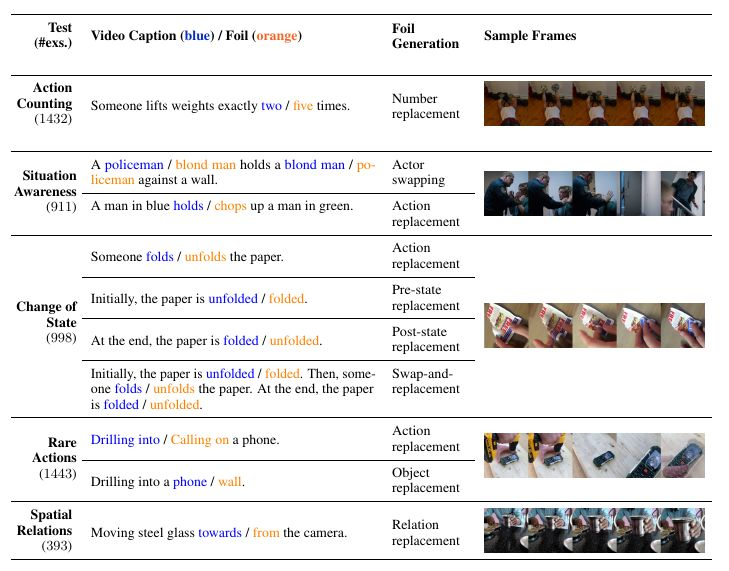
\includegraphics[width=0.65\textwidth]{vilma_test}
    \caption{The VILMA tests on VidLMs \cite[Table 1]{kesen2023ViLMA}.}
    \label{fig:vilma_test}
\end{figure}

Structure of each main test \cite{kesen2023ViLMA}:
{\it 
\begin{structure}

\begin{enumerate} \label{test_structure}
\item In step 1, be harvested high-quality examples from existing \textbf{video-language datasets}.
\item In step 2, be created counterfactual examples or ‘\textbf{foils}’, so that a test requires distinguishing correct from counterfactual video+text pairs.
\item In step 3, be created a \textbf{Proficiency test} to gauge if a model learns the capabilities we deem necessary to solve the main test.
\item In step 4, be applyed automatic and manual validation of the examples and their counterfactuals to control for biases and to ensure a high-quality evaluation benchmark.
\item Finally step, be tested whether existing VidLMs can solve the \textbf{Proficiency tests} and distinguish correct from counterfactual examples in the main tests.
\end{enumerate}
\end{structure}

}

Explanation of the Tests of VILMA:

Here, I explain how the tests work. In step 1 of the structure \ref{test_structure}, the choice of dataset is mentioned. I will not mention these since in this report I am focusing on explaining the functionalities and objectives of these tests. That said, each test uses a different dataset with specialized annotations for the purpose of the test (for more information review \cite{kesen2023ViLMA}).

\subsubsection{PROFICIENCY TESTS:}
\textbf{Brief definition:}
It is a preliminary test for the main tests. This test will be called with different objectives from the main tests.

This test computes the capacity of the model (VidML) to solve simple visuo-linguistic tasks, that do not have a demanding temporal model for this test.

This test is useful to rule out if there is bias in a model, for example, when a VidML passes the main test, but not the \textbf{Proficiency test}, then there should be bias in the VidML.

Thus, as this test will be called by all main tests, it is important to mention that not all \textbf{Proficiency test} objectives are useful for all main tests, below are the objectives for each main test \cite{lei2021clipbert}:

Objectives for \textbf{Spatial Relation}, \textbf{Change State} and \textbf{Situation Awareness} test:
The objective is to identify objects mentioned in a caption.

Objectives for \textbf{Action Counting} and \textbf{Rare Action} test:
The objective is to recognize actions in a caption and validate existence of objects (objects on which some action falls and subjects who perform it) in the frame respectively.

\textbf{Procedure of Proficiency test is:}
The SpaCy dependency parser is used to identify \textit{target words} (verbs for actions and nouns for objects) and mask them (the mask is a type of tokenization). Then the \textit{target words} are replaced by \textit{foil words} generated with \textbf{Masked Language Modeling (MLM)} using RoBERTa or T5, generate 3 \textit{words foil}, which gives us 3 \textit{foil captions}.

To validate the \textit{words foils} applying an ALBERT 10 model finetuned on \textbf{Natural Language Inference (NLI)}. ALBERT 10 model is used to discard \textit{words foils} that are entailed (E) by the \textit{original caption}, that mean, these \textit{foil words} do not change the meaning of the \textit{caption}, because the \textit{foil caption} should not coincide with the frame that represents the \textit{original caption}, \textit{foil words} that are neutral (N) or contradictory (C) be accepted as \textit{foil words candidates}.

The second validation for \textit{foil words candidates} is the \textbf{GRUEN} score. The \textbf{GRUEN} score is calculated through \textbf{BERT} model finetuned on the \textbf{Corpus of Linguistic Acceptability (CoLA)}. \textbf{GRUEN} rejects samples smaller than a pre-established threshold.

If none of the \textit{foil words} pass both steps (NLI and CoLA), that \textit{caption} si discarted.

\subsubsection{ACTION COUNTING:}
\textbf{Brief definition:} Measures the ability to accurately count the actions that occur in the video.

\textbf{Structure \ref{test_structure}:}
\begin{itemize}
\item Step 1: specialized dataset
\item Step 2:
\begin{itemize}
\item First, the actions are noted at the end of the action, along with the frame number in which it ended. A structure is created to note the number of times the action is repeated, such as “someone performs exactly $<$number$>$ push-ups” and the $<$number$>$ value is called \textit{placeholder}.
\item Second, the \textbf{placeholder} of \textit{caption} be annotated with the correct value of repetitions of the action.
\item Third, \textit{Foil-captions} are generated by changing the \textit{placeholder number}, the \textit{foil-caption} with placeholder that exceed the maximum value of all the actions perform in the video are discarded. In other words, among all the actions performed in the video, it counts how many times the most frequent action is repeated. This is done in two subtests.
\begin{itemize}
\item In the first subtest called \textbf{easy}, an incorrect number of \textbf{placeholder number} of caption should be put, the incorrect values would be the values of the most frequent actions (a frequent action is the times the same action is repeated).
\item In the second subset called \textbf{difficult}, the \textit{caption} no longer used, now the \textbf{foil-captions} generated by the \textbf{Proficiency test} are used (step 3), the \textit{foil captions} be added the \textit{placeholders} with the values of the most frequent actions.
\end{itemize}
\end{itemize} 
\item Step 3: The objective of the \textbf{Proficiency test} for this test is to find actions, but to use \textbf{Proficiency test} the caption should change its structure, for example if it is like this ``a man performs exactly $<$number$>$ push-ups" it should be replaced by ``a man performs push-ups". Having the \textit{captions}, now the \textit{foil-captions} are generated:
\begin{itemize}
\item First the \textbf{Proficiency test} is used for the verbs, but the \textit{captions} that have personal pronouns (like I, they, etc) and conjunctions (like and, but, etc.) are discarded.
\item Second, the \textbf{Proficiency test} is used for nouns.
\item Third, \textit{caption} that are not valid in the video only should selected for that, the folowing steps should done:
\begin{enumerate}
\item \textit{Captions with similar actions} in other videos in the dataset be search.
\item The verbs and nouns of the \textit{caption} are replaced with those of the \textit{captions with similar actions}.
\item A \textit{perplexity evaluation} is applied to the \textit{foil-captions} to discard meaningless captions.
\item Finally, \textit{foil-captions} are taken at random from all \textit{foil-captions} generate.
\end{enumerate}
\end{itemize}

\item Step 4: A manual review of the \textit{foil-captions} and \textit{captions} is carried out.
\item Step 5: The \textit{foil-captions} are entered into VidML, and their results are reviewed.
\end{itemize}

With this test we can see if the VidML is not biased by the most frequent number of actions.

\subsubsection{SITUATION AWARENESS:}
\textbf{Brief definition:}
This test measures if the VidLM is aware of the actors and objects involved in an action. For example, if someone writes with a pen, then that pen should exist in the video.
This test is divided in 2 tests:
\begin{itemize}
\item \textbf{Action Replacement:} This test evaluates the efficiency of the VidLM in distinguishing actions in a video sequence. For this, a \textit{caption} should be taken and a \textit{copy} is created of it, but the action (verb) of \textit{copy} is changed.
\item \textbf{Actor Swapping:} This test aims to recognize actors (someone performing an action) and objects on which an action is performed inside a video sequence. For this, a \textit{caption} should be taken and a \textit{copy} is created of it, but replace its actors and objects.
\end{itemize}
Following \textbf{Structure \ref{test_structure}:}
\begin{itemize}
\item Step 1: Specialized dataset
\item Step 2: \textit{foil-captions} are obtained by Subtests \textbf{Action Replacement} and \textbf{Actor Swapping}.
\item Step 3: For this test, the \textbf{Proficiency test} focuses on finding the identified \textit{objects} and \textit{actors} and so in step 4 be able to compare these \textit{object} with the \textit{foil-captions objects} created by the subtests of step 2.
\item Step 4: A manual review of the \textit{foil-captions} and \textit{captions} is carried out.
\item Step 5: The \textit{foil-captions} are entered into VidML, and their results are reviewed.
\end{itemize}
\subsubsection{CHANGE OF STATE:}
\textbf{Brief definition:}
This test measures whether the model is aware of the implications of an action, such as:
\begin{itemize}
\item The action of walking: implies that someone is standing up, nobody can walk while sitting down. 
\item The action closing a door: implies that the door is open.
\end{itemize}

The test needs a set of verbs with their grammatical implications and preconditions to perform an action, these verbs are called \textit{change of state (CoS) verbs}. These \textit{CoS verbs} are stored in a tuple of dimension 4 ([pre-state, verb, pos-state, reverse verb]), such as [open, to close, closed, to open].

Then, the \textit{captions} of the VidLM dataset that contain the \textit{CoS verbs} are searched, these will be named \textit{candidate captions}.

Then, the \textit{candidate captions} are rebuilded the following \textbf{VILMA} structure, which differentiates the transitive verbs (verbs that also affect objects) from the intransitive verbs (which only affect the subject):

\begin{structure}
\begin{itemize} \label{cos_structure}
\item \textbf{Action caption template:} “Someone $<$change-of-state-verb$>$ the $<$object$>$.” for transitive change-of-state verbs, “The $<$subject$>$ $<$change-state-verb$>$.” for intransitive ones.
\item \textbf{Pre-State caption template:} “Initially, the $<$subject/object$>$ is $<$pre-state$>$.”;
\item \textbf{Post-State caption template:} “At the end, the $<$subject/object$>$ is $<$post-state$>$.”;
\item \textbf{Reverse caption template:} “Initially, the $<$object$>$ is $<$pre-state$>$. Then someone $<$change- state-verb$>$ the $<$object$>$. At the end, the $<$object$>$ is $<$post-state$>$.” for transitive change- of-state-verbs. “Initially, the $<$subject$>$ is $<$pre-state$>$. Then the $<$subject$>$ $<$change-state- verb$>$. At the end, the $<$subject$>$ is $<$post-state$>$.” for intransitive ones.
\end{itemize}
\end{structure}


Therefore, the \textbf{action caption template} and the \textbf{reverse caption template} are the \textit{foil-captions}.

Following \textbf{Structure \ref{test_structure}:}
\begin{itemize}
\item Step 1: Specialized dataset
\item Step 2: The \textit{foil-captions} are obtained, with the structure \ref{cos_structure}.
\item Step 3: For this test, \textbf{Proficiency test} focus only on the detection of objects or actors, depending on whether it is a transitive verb or not. If the verb is transitive then \textbf{Proficiency test} detects objects and actors, and if the verb is not transitive then \textbf{Proficiency test} detects only actors.
\item Step 4: A manual review of the \textit{foil-captions} and \textit{captions} is carried out.
\item Step 5: The \textit{foil-captions} are entered into VidML, and their results are reviewed.
\end{itemize}

\subsubsection{RARE ACTIONS:}
\textbf{Brief definition:}
The objective of this test is measuring VidLM's ability to identify novel compositions or unusual compositions, for example "cutting a computer keyboard with a chainsaw".

This test requires that the unusual events should described using a \textit{verb-noun pair}, for example “cutting a keyboard.” These descriptions should not have an actor.

The test is divided in two subtests:
\begin{itemize}
\item \textbf{Action Replacement:} The verbs within caption should replaced by another that can accommodate this situation such as “typing on the keyboard”.
\item \textbf{Object Replacement:} The objects within caption should replaced by others objects found in the video,  to be more specific, the other objects found should be within a range of 8 frames from where the frame of the original caption.
\end{itemize}
These two subtests \textbf{Action Replacement} and \textbf{Object Replacement} return the foil-captions.

Again, following \textbf{Structure \ref{test_structure}:}
\begin{itemize}
\item Step 1: Specialized dataset.
\item Step 2: The \textit{foil-captions} are obtained by \textbf{Action Replacement} and \textbf{Object Replacement} subtests.
\item Step 3: For the \textbf{Rare Action test}, \textbf{Proficiency test} only focus on finding the objects, and the object within foil-captions no long replaced by any object, but it will be some objects found in 8 frames around the orignal caption frame.
\item Step 4: A manual review of the \textit{foil-captions} and \textit{captions} is carried out.
\item Step 5: The \textit{foil-captions} are entered into VidML, and their results are reviewed.
\end{itemize}

\subsubsection{SPATIAL RELATIONS:}
The objective of this test is to measure the ability of a VidLM to understand spatial relations as spatio-temporal relations (prepositions) in a video, such as ``moving something towards or from something".

For this test, \textit{caption} that contain a spatial or spatio-temporal relations should be looked for within the dataset of the \textbf{VidML} (I will call it a set of captions).

Then, the \textit{foil-captions} should created, a \textit{foil-caption} is created as follows:
A \textit{copy of a caption} is created, then replace its prepotions in the \textit{copy} with the prepotions from the set of \textit{captions}. Then, a \textit{perplexity test} is performed on the copy and if the \textit{copy} passes the test it would be a valid \textit{foil-caption}.

Then,the 10 \textit{foil-captions} are taken and pass them over an \textbf{NLI} model, the neutral and contradictory \textit{foil-caption} are kept, the rest is discarted. Then, the \textbf{GRUEN} score is calculated to discard some more.
Then the remaining \textit{foil-captions} will be the \textit{foil-captions candidates}.

Following \textbf{Structure \ref{test_structure}:}
\begin{itemize}
\item Step 1: Specialized dataset
\item Step 2: The \textit{foil-captions} are obtained as indicated above..
\item Step 3: For this test,the \textbf{Proficiency test} only focuses on identifying the objects in the \textit{caption}, similar to the \textbf{Proficiency test} carried out for the \textbf{Change of Status test}.
\item Step 4: A manual review of the \textit{foil-captions} and \textit{captions} is carried out.
\item Step 5: The \textit{foil-captions} are entered into VidML, and their results are reviewed.
\end{itemize}

